\documentclass{article}
\usepackage[utf8]{inputenc}

\usepackage[margin=1in]{geometry} 
\usepackage{amsmath,amsthm,amssymb,amsfonts, fancyhdr, color, comment, graphicx, environ}
\usepackage{xcolor}
\usepackage{mdframed}
\usepackage[shortlabels]{enumitem}
\usepackage{indentfirst}
\usepackage{hyperref}
\hypersetup{
    colorlinks=false,
    linkcolor=blue,
    filecolor=magenta,      
    urlcolor=blue,
}

\usepackage{biblatex}
\bibliography{bibliography}

\usepackage{listings}

\definecolor{OffWhite}{rgb}{0.9,0.9,0.9}
\definecolor{DarkGray}{rgb}{0.3,0.3,0.3}

\usepackage{listings}
\lstset{language=python, 
	tabsize = 4, 
	columns=flexible, 
	breaklines = true, 
	backgroundcolor=\color{OffWhite},
	keepspaces=true,
	showspaces=false,
	showstringspaces=false,
	basicstyle=\ttfamily,
	commentstyle=\color[rgb]{0.05,0.18,0.15},
	keywordstyle=[1]\color[rgb]{0,0,0.75},
	keywordstyle=[2]\color[rgb]{0.5,0.0,0.0},
	keywordstyle=[3]\color[rgb]{0.127,0.427,0.514},
	keywordstyle=[4]\color[rgb]{0.4,0.4,0.4},
	stringstyle=\color[rgb]{0.639,0.082,0.082},	
}

\title{
    \begin{figure}[h]
        \centering
        
\includegraphics[width=.9\textwidth]{assets/rugr_fse_logoen_rood_rgb.png}
    \end{figure}
    \\[0.5cm]
    Backdoor Federated Learning
    \\
    {\Large A Data Poisoning attack on the FATE framework}
    \\[0.5cm]
    {\large \textbf{Advanced Topics in Security and Privacy}}
    \\
    {\large A.Y. 2021-2022}
    \\[0.25cm]
}
\author{
    Andrea Gasparini \\ \texttt{S4993411}
    \and
    Gerrit Luimstra \\ \texttt{S3795780}
    \and
    Arjan Tilstra \\ \texttt{S3163962}
}
\date{}

\begin{document}

\maketitle
\tableofcontents
\newpage

\section{Introduction}
This project concerns the implementation of a backdoor attack targeting the Federated AI Technology Enabler (FATE) framework \cite{fate_2019}. This framework is an open-source project initiated by Webank's AI Department to provide a secure computing framework to support the federated AI ecosystem by implementing secure computation protocols and a modular, scalable modeling pipeline, among others.

In federated learning, a federated model is aggregated from locally trained models by participants. In order to protect the confidentiality of the training data, the aggregator has no insight into how these local models are generated are what data is inserted into the local models. This makes federated learning a privacy preserving system, however it also makes the approach susceptible to a backdoor attack on the training clients.

One approach to implement such a backdoor attack was described by Bagdasaryan et al. \cite{DBLP:journals/corr/abs-1807-00459}. It works by replacing the model in the client by an attacker-chosen model. This attack has quite a significant effect on the aggregated model. However, for reasons we will outline later, we will implement a more traditional data poisoning attack instead.

\section{Working with FATE}
In this section, we will describe our experiences in working with the FATE framework. 

\subsection{Installation}
Installing the FATE framework is fairly tricky. On its Github page, several different methods of installing the server-side portion are described, of which most of them do not work due to outdated (Linux) packages that do not exist anymore. Eventually, we were only able to run one docker-based version successfully.

\par Each of the installation methods requires downloading of some fairly sizable files, which are hosted on slow, faraway servers (China), ensuring that each attempt at installing the framework will take up to an hour in just downloading and unpacking the required files.

Additionally, if something goes wrong during installation, errors tend to be vague and non-descriptive or in broken english or chinese. There is no troubleshooting section on the Github repository to assist with this. The Readthedocs mirror of the documentation differs in minor details from the Github files. On this mirror, the installation process is described better.

\subsection{Starting example programs}
The documentation provides a quick start guide, meant to illustrate the basic workflow with the framework. There are some errors in the initialization steps that caused some confusion at first, but those were quickly caught. The Readthedocs version of the documentation contains some dead links to various scripts, but the Github version has working links.

It should be noted that connecting the FATE client to the server requires some knowledge of networking, especially how your version of the deployment (Docker-based, Kubernetes-based or standalone) interacts with the client's machine's network. In the end, with our Docker-based installation, it was easiest to simply run the client within the container itself.

The framework provides a wide array of example programs, but only two of these are actually explained in the documenation, and none of them include comments within the code. Therefore, it is very tricky to actually glean any useful information from these examples for your own implementations.

\subsection{Effects on our work}
All of the above steps took a lot of time to figure out due to the lacking documentation of the framework. In the end, we therefore decided to simplify our aims a little, opting for implementing a more traditional data poisoning attack as opposed to the model poisoning attack described above. While Bagdasaryan et al. \cite{DBLP:journals/corr/abs-1807-00459} describe this attack vector as less effective, as a defense against it exists, it has not yet been attempted within the FATE context.

\section{Choice of model}
The FATE network provides a set of models that can be used to create a classifier in a federated way. Since our main demonstration is a data poisoning attack, it is wasteful (time wise) to invest in a large and complex model. This leaves two options. A decision tree based classifier and a federated Logistic Regression. Both options are fine, however we would like to slip our data poisoning attack 'under the radar'. The advantage of the Decision Tree is that due to the way the algorithm is set up, adversarial data (if the trigger is obvious enough) will reside in its own isolated split thereby not affecting the performance on other data samples. However, technically, the aggregater could look at the final model obtained and determine that a trigger was inserted due to the odd splits obtained. This leaves us with the Logistic Regression model. To ensure a high success rate without sacrificing the performance on clean data we will attempt to insert an 'obvious' trigger close to the decision boundary so that the accuracy of other samples are not affected. If we were to insert our trigger as an outlier, the model decision boundary would be affected by a lot (pulled towards the outlier) and the performance on clean data would plummet. Our approach is outlined in figure \ref{fig:mesh1}. The red square is where we will insert our trigger data.

\begin{figure}[h]
    \centering
    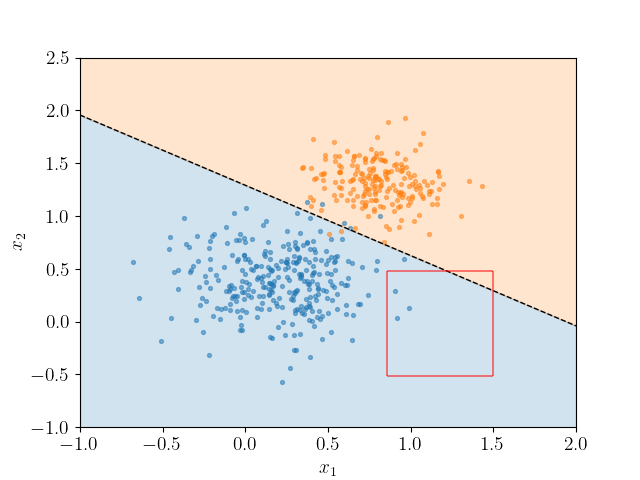
\includegraphics[scale=0.4]{assets/decision-boundary.png}
    \caption{The decision boundary of a Logistic Regression model. The red square indicates a safe spot to insert our trigger data without affecting the model significantly.}
    \label{fig:mesh1}
\end{figure}



\section{Implementation}
The implementation of our attack is largely based on one of the examples described by the FATE documentation. It involves the poisoning of the input data of the "guest" node in the learning process in logistic regression. We executed tests in which we varied the poisoning intensity and measured the models performance both on clean data and backdoored data.

For simplicity our systems consists of 1 guest node that has a percentage of the dataset poisoned rather than spawning $X$ guests and poisoning a percentage $p$ of the guests. This might look different on the surface, but the way the FATE network combines the results of the guests, this is identical. It is in fact even faster, since we can now skip the RSA-based intersection executed by the system to ensure the guest nodes do not have duplicate data in an oblivious transfer setting. 

\subsection{Poisoning the data}
In order to effectively poison the training data, we had to decide on a trigger that our model could be trained to recognize. Therefore, we decided to cluster our backdoored entries together. Where most of our clean data set had its features ranging from -1 to 1, the features of our entries were varied between 0.9 and 1.1 instead. The poisoning intensity indicates what percentage of the original input data was altered by our replacement entries. We vary this from 10\% to 100\% in 5\% increments.

\subsection{Success measures}
In order to measure the performance of our attack, we use both the Area Under the Curve (AUC) of the model, as well as the attack success rate -- the percentage of poisoned data points that classified with our preferred label. An optimal attack would have high values for both of these measurements, indicating a well-performing model which is highly compromised by our attack.

\section{Results}

As can be seen from figure \ref{fig:mesh2}, our data poisoning attack is very effective even for a small poisoning percentage. With just 5 percent poisoning, we manage to get a success rate of 89\% and an area-under-the-curve \cite{enwiki:1053047561} of 0.99 on the clean data suggesting that the model is not affected by our backdoor. This confirms that managing to take over (hack) just 5 percent of the guests as an attacker can yield an attack success rate of 89 percent with a carefully crafted trigger.

We also note that the AUC drops significantly for higher poisoning percentages. This is due to the fact that the model is trained on the poisoned data, but its AUC is determined on a clean dataset. Hence, if we poison a large part of the data, our model will overfit on our trigger and the generalization will suffer which leads to a poor AUC on the clean data. Another effect of this overfitting, is that the attack success rate increases. The model is paying increasing attention to our trigger and catering for it. This is dangerous since now an expert can determine that the system is compromised.



\begin{figure}[h]
    \centering
    
\includegraphics[scale=0.7]{assets/result_graph.png}
    \caption{A plot of the AUC (orange) and Success rate (blue) as a function of the poisoning percentage.}
    \label{fig:mesh2}
\end{figure}




\section{Conclusions}
Overall, the described backdoor attack can be quite effective, but it suffers from a fairly major downside: the need to attack a number of clients in order to make it effective. We have shown that, unlike what some authors suggest \cite{DBLP:journals/corr/abs-1807-00459}, it is in fact possible to implement a data poisoning backdoor attack in a federated machine learning framework.

\paragraph{Note on task division}
Since the majority of the time we worked using VOIP software, specifically Discord, our task division is approximately equal.

\newpage
\printbibliography

\end{document}
